\documentclass[11pt,french]{article}
\usepackage[autolanguage]{numprint}
\usepackage{babel}
\usepackage[utf8]{inputenc}
\usepackage[T1]{fontenc}
\usepackage{graphicx}

\usepackage{geometry,graphicx,hyperref,amsmath,amsfonts,physics,amssymb,bm,mathtools}
%\usepackage{icomma}
\usepackage{colordoc}
\usepackage{ragged2e}
\usepackage{amsmath}
\usepackage{hyperref}
\hypersetup{
    colorlinks=true,
    linkcolor=blue,
    filecolor=magenta,      
    urlcolor=cyan,
    pdfpagemode=FullScreen
    }
\urlstyle{same}
\date{}
\title{\textbf{\color{blue}La Géométrie de l'Information: une introduction concrète et simple}}
\author{M. A. G. Decastro\\}
	
	 
	 
\begin{document}
	\maketitle

\renewcommand{\abstractname}{Résumé}
	
\begin{abstract}
La théorie moderne de la Géométrie de l'Information (ou \textit{Information Geometry}, en anglais) est un domaine interdisciplinaire des mathématiques combinant la géométrie riemannienne, la théorie de l'information et la statistique initiée en grande partie par les travaux du mathématicien japonais Shun-ichi Amari (voir \cite{amari1985differential}). Elle suscite un certain intérêt ces dernières années du fait de ses champs d'application notamment dans le domaine de l'apprentissage machine. Tel qu'indiqué par le titre, cet article se veut une introduction pratique, simple et accessible pour un étudiant en fin de baccalauréat en mathématiques. Après un rappel de quelques outils de géométrie riemannienne, des exemples calculatoires sont présentés afin de montrer comment utiliser quelques uns des concepts majeurs de la Géométrie de l'Information dans les sections suivantes. La structure de cet article s'inspire beaucoup du livre \cite{calin2014geometric}.
	 	
\end{abstract}
\nocite{*}
\section{Notions élémentaires de géométrie riemannienne}
En Géométrie de l'Information, le cadre d'étude est la variété riemannienne. En supposant connu les notions élémentaires de topologie et sans rentrer dans les subtilités de la théorie des variétés différentielles, explicitons d'abord ce qu'on entend par variété topologique puis variété différentielle et finalement variété riemannienne en introduisant informellement et au besoin d'autres définitions.\\

Une variété topologique $M$ est un espace topologique de \textit{Hausdorff} éventuellement \textit{à base dénombrable} et tel que pour \textbf{tout} point $p\in M$ il existe un couple $(U, \phi)$, appelé carte où $U\subset M$, $p \in U$, $\phi:U \longrightarrow U^{'}$ homéomorphisme et $U^{'}$ ouvert de $\mathbb{R}^{n}$.  
On appelle dimension de $M$ le plus petit $n$ tel que la condition précédente est vraie et $atlas$ de $M$ une famille de cartes dont les domaines $U$ recouvrent $M$.

Deux cartes $(U, \phi)$ et $(V, \psi)$ seront dites compatibles si $U \cap V=\emptyset$ ou bien $U\cap V\neq \emptyset$ et que \textit{les applications de changement de cartes} $\phi\circ\psi^{-1}$ et $\psi\circ\phi^{-1}$ sont des $C^{k}$-difféomorphismes pour tout $k\geq 1$. Lorsque toutes les cartes compatibles à un atlas font déjà partie de l'atlas celui-ci est dit maximal et on le qualifie alors de structure différentiable\footnote{On dit aussi structure différentielle}.

Une variété topologique devient une variété différentielle lorsqu'elle est munie d'une structure différentiable. \\ 

Un exemple standard de variété différentielle est la sphère: 

\begin{equation*}
    \mathbb{S}^n=\{u=(u_1, u_2,\cdots, u_{n+1}) \in\mathbb{R}^{n+1}\mid\sqrt{u_1^2+u_2^2+\cdots+u_{n+1}^2}=1\}
\end{equation*}
Son atlas peut être constitué uniquement de deux cartes $\left(U, \phi_N \right)$ et $\left (V, \phi_S \right)$ où $U\cap V \neq \emptyset$ et $\phi_N$ et $\phi_S$ sont des projections stéréographiques définies par:
\begin{align*}
\phi_N\colon\mathbb{S}^n\setminus{N}&\longrightarrow\mathbb{R}^n &\text{et} \quad\phi_S\colon\mathbb{S}^n\setminus{S}&\longrightarrow\mathbb{R}^n\\
   u &\longmapsto\phi_N(u)=\frac{(u_1, u_2,\cdots, u_n)}{1-u_{n+1}}  &  u&\longmapsto\phi_S(u)=\frac{(u_1, u_2,\cdots, u_n)}{1+u_{n+1}}
\end{align*}
avec $N=(1, 0, \cdots, 0)$ et $S=(0, \cdots, 0, -1)$ comme centres de projection.

Notons que les applications $\phi_N$ et $\phi_S$ sont des homéomorphismes d'inverses
\begin{equation*}
\phi_N^{-1}(x)=\frac{\left (2x_1, 2x_2, \cdots, 2x_n, \norm{x}^2-1\right)}{\norm{x}^2+1}=\phi_S^{-1}(x)\quad\text{et que}\quad \phi_N\circ\phi_S^{-1}(y)=\frac{x}{\norm{x}^2}=\phi_S\circ\phi_N^{-1}   
\end{equation*}
sont bien des $C^{k}$-difféomorphismes pour tout $x\;\text{et}\;y\;\text{dans}\;\mathbb{R}^n\setminus\{0\}$.\\

Finalement,  $M$ est une variété riemannienne de dimension $n$ si elle est munie d'une métrique riemannienne ou tenseur métrique, c'est-à-dire d'une forme bilinéaire\footnote{Donc ayant une représentation matricielle de dimension $n\times n$.}, symétrique et définie positive $g$ qui en tout point $p\in M$ et à tout couple $(A, B)$ de vecteurs appartenenant à l'espace des vecteurs tangents à $M$ au point $p$ associe un réel $g(A, B)$. Si de plus $(X, Y)$ est un couple de champs de vecteurs differentiables sur un ouvert contenant $p$ alors la fonction $g(X_p, Y_p)$ est différentiable.

Les composantes de la métrique riemannienne, c'est-à-dire les entrées de la matrice associée, s'obtiennent en considérant d'abord le champs de base $(X_p^1, X_p^2, \cdots, X_p^n)$ associé à une carte puis en calculant $g_{ij}=g(X_p^i, X_p^j)$ pour $i,j=1,2,\cdots, n.$ Il y a en tout $n\times  n$ fonctions composantes. Ces dernières sont utilisées pour calculer les \textit{symboles de Christoffel}:
\begin{equation}\label{christoffel_symbs}
    \Gamma_{ij,k}=\frac{1}{2}\left(\frac{\partial g_{jk}}{\partial\xi_{i}}+\frac{\partial g_{ik}}{\partial\xi_{j}}-\frac{\partial g_{ij}}{\partial\xi_{k}}\right) \quad\text{et}\quad \Gamma_{ij}^k=\sum_{l=1}^n\Gamma_{ij, l}g^{lk} \quad\text{avec}\quad i,j,k=1,2, \cdots, n.
\end{equation}
où les $ \partial g_{ij}/\partial\xi_k$ sont obtenus directement par différentiation et $g^{lk}$ correspond à la $lk$-ième composante de l'inverse de la métrique riemannienne.

Ces symboles (en réalité des fonctions) sont à leur tour utilisés pour calculer une \textit{géodésique} que nous présentons au paragraphe suivant.
\newline

La géodésique est l'un des concepts les plus importants en géométrie riemannienne. Elle permet de déterminer le plus court chemin entre deux points d'une variété. Soit une courbe differentiable sur $D\subset M$, c'est-à-dire une application $c\colon I\subset\mathbb{R}\longrightarrow M$ pour laquelle on peut trouver une carte $(U, \phi)$ de $M$ de champs de base associé  $(X_p^1, X_p^2, \cdots, X_p^n)$ avec $U\subset D,\quad p\in U$ et telle que $c\circ\phi^{-1}\colon\phi(U)\longrightarrow\mathbb{R}$ soit différentiable. 
Si on suppose que $g(X_p^i, X_p^j)=\delta_{ij}$ et que $\partial g_{ij(p)}/\partial X_p^i=0$ alors il existe une application dérivée $D/dt$ \footnote{En réalité, on appelle cette application une \textit{connexion de Levi-Civita.}} telle que $\frac{D}{dt}\left(\frac{d}{dt}c(t)\right)=0$ pour tout $t\in I$. En d'autres termes, l'accélération est nulle partout sur cette courbe. On appelle une telle courbe une géodésique. Fonctionnellement, cette dérivée seconde détermine un système d'équations différentielles du second ordre dont la (ou les) solution(s) donne(ent) exactement les fonctions composantes de la courbe du plus court chemin:\\
\begin{equation}\label{geodesics_equn}
    \frac{d^2c_k(t)}{dt^2}+ \sum_{i,j=1}^n \Gamma_{ij}^k\frac{dc_i(t)}{dt}\frac{dc_j(t)}{dt}=0\quad \text{avec}\quad k=1, 2, \cdots, n
\end{equation}
Ici, $c_k(t)$ est la $k$-ième fonction coordonnée de la courbe $c(t)$. Idem pour $c_i(t)$ et $c_j(t)$.\\

Dans la section suivante, nous aurons l'occasion de calculer une métrique riemannienne, des \textit{symboles de Christoffel} ainsi qu'une géodésique.\\


\section{Métrique de Fisher et géodésiques associées} 
Considérons maintenant une famille de distributions normales paramétrées par deux variables, une moyenne $\mu$ et un écart-type $\sigma$:
\begin{equation}\label{my_manifold}
	S=\{p_{\xi}=p(x;\xi)=p_{\xi}(x) \mid \xi=(\mu, \sigma^2)\in\mathbb{R} \times ]{ 0,+\infty[} \text{ et } x\in\mathbb{R}\}, 
\end{equation}
où $p_{\xi}$ est une distribution normale de densité $\frac{1}{\sigma\sqrt{2\pi}}\exp\left(-\frac{(x-\mu)^2}{2\sigma^2}\right)$ et $\xi$ le vecteur des paramètres $\mu$ et $\sigma$. 

Puisque $\mu\times\sigma\in\mathbb{R} \times ]{0,+\infty[}$ et qu'ils paramètrent toute la surface $S$ alors pour tout point $p_{\xi}\in S$ il est raisonnable de penser qu'  on peut trouver un homéomorphisme entre un ouvert contenant $p_{\xi}$ et un ouvert de $\mathbb{R} \times ]{0,+\infty[}$. De plus, la fonction de densité est infiniment différentiable par rapport aux paramètres. On peut donc supposer aisément que $S$ est une variété différentielle où le système de coordonnées est donné par l'application $\phi(p_{\xi})=\xi$.\\

En géométrie de l'information, une métrique riemannienne naturelle très utilisée est l'information de Fisher (voir \cite[Proposition 1.7.1]{calin2014geometric}) dont les composantes sont données par  :
\begin{equation*}
	g_{ij}(\xi):= -E\left[\frac{\partial^2\ln(p_{\xi}(x))}{\partial\xi_j\partial\xi_i}\right]=-\int_{\mathbb{R}}\frac{\partial^2\ln(p_{\xi}(x))}{\partial\xi_j\partial\xi_i}p_{\xi}(x)dx \quad i,j=1,2
\end{equation*}  
où $E$ est l'espérance mathématique, \text{ln} le logarithme népérien et $\partial/\partial\xi_i$ la dérivée par rapport au paramètre $\xi_i$.

Sachant que $\int_{-\infty}^{+\infty}p_{\xi}(x)dx=1$ et en prenant $\xi_1=\mu$ et $\xi_2=\sigma$, on calcule aisément chacune de ses composantes:

    \begin{align*}
    g_{11}&=-\int_{-\infty}^{+\infty}\frac{\partial^2\ln(p_{\xi}(x))}{\partial\mu^2}p_{\xi}(x)dx=-\int_{-\infty}^{+\infty}-\frac{1}{\sigma^2}p_{\xi}(x)dx=\frac{1}{\sigma^2}\int_{-\infty}^{+\infty}p_{\xi}(x)dx=\frac{1}{\sigma^2}
    \\
    g_{12}&=g_{21}=-\int_{-\infty}^{+\infty}\frac{\partial^2\ln(p_{\xi}(x))}{\partial\sigma\partial\mu}p_{\xi}(x)dx=\int_{-\infty}^{+\infty}\frac{2(x-\mu)}{\sigma^3}\frac{1}{\sigma\sqrt{2\pi}}\exp\left(-\frac{(x-\mu)^2}{2\sigma^2}\right)dx\\
    &=\frac{2}{\sigma^2\sqrt{2\pi}}\int_{-\infty}^{+\infty}\frac{(x-\mu)}{\sigma^2}\exp\left(-\frac{(x-\mu)^2}{2\sigma^2}\right)dx=-\frac{2}{\sigma^2\sqrt{2\pi}}\left[\left.\exp\left(-\frac{(x-\mu)^2}{2\sigma^2}\right)\right|_
    {-\infty}^{+\infty}\right]=0\\
    g_{22}&=-\int_{-\infty}^{+\infty}\frac{\partial^2\ln(p_{\xi}(x))}{\partial\sigma^2}p_{\xi}(x)dx=-\int_{-\infty}^{+\infty}\left (\frac{1}{\sigma^3\sqrt{2\pi}}+\frac{3(x-\mu)^2}{\sigma^5\sqrt{2\pi}}\right)\exp\left(-\frac{(x-\mu)^2}{2\sigma^2}\right)dx\\
    &=-\frac{1}{\sigma^2}
    -\frac{3}{\sigma\sqrt{2\pi}}\left[\left.\frac{-(x-\mu)}{2\sigma^2}\exp\left(-\frac{(x-\mu)^2}{2\sigma^2}\right)\right|_{-\infty}^{+\infty}\right]+\frac{3}{\sigma^3\sqrt{2\pi}}\int_{-\infty}^{+\infty}\exp\left(-\frac{(x-\mu)^2}{2\sigma^2}\right)dx\\
    &=-\frac{1}{\sigma^2}+\frac{3\sqrt{2\pi\sigma}}{\sigma^2\sqrt{2\pi\sigma}}=\frac{2}{\sigma^2}
    \end{align*} 
On peut les regrouper dans la  matrice $\mathbf{g}_{ij}$ suivante dite matrice d'information de Fisher:
\begin{align*}
\mathbf{g}_{ij}
&=
    \begin{bmatrix}
    \dfrac{1}{\sigma^2} & 0
    \\[9pt]
    0 & \dfrac{2}{\sigma^2}
    \end{bmatrix}
\end{align*}\\

Notons tout de suite que dans les calculs qui suivent $k$ prendra les valeurs 1 et 2, en référence respectivement à $\mu$ et $\sigma$ considérés à la fois comme éléments du champs de base et comme fonctions composantes.\\

En retenant les mêmes notations on a que:
\begin{align*}
    \frac{\partial g_{11}}{\partial\mu}=\frac{\partial g_{12}}{\partial\mu}=\frac{\partial g_{12}}{\partial\sigma}=\frac{\partial g_{21}}{\partial\mu}
    &=\frac{\partial g_{21}}{\partial\sigma}=\frac{\partial g_{22}}{\partial\mu}=0, \quad
    \frac{\partial g_{11}}{\partial\sigma}=\frac{-2}{\sigma^3} \quad \text{et} \quad
    \frac{\partial g_{22}}{\partial\sigma}=\frac{-4}{\sigma^3}.
\end{align*}

Et en utilisant \eqref{christoffel_symbs} les symboles de Christoffel non-nuls sont alors:
\begin{equation*}
    \Gamma_{12,1}=\Gamma_{21,1}=-\frac{1}{\sigma^3},\quad \Gamma_{11,2}=\frac{1}{\sigma^3}, \quad \Gamma_{22,2}=-\frac{2}{\sigma^3}
\end{equation*}
et 
\begin{align*}
    \Gamma_{12}^1&=\Gamma_{12,1}g^{11}+\Gamma_{12,2}g^{21}=-\frac{1}{\sigma^3}\sigma^2=-\frac{1}{\sigma}\\
    \Gamma_{21}^1&=\Gamma_{21,1}g^{11}+\Gamma_{21,2}g^{21}=\frac{1}{2}\left(-\frac{2}{\sigma^3}\right)=-\frac{1}{\sigma}\\
    \Gamma_{11}^2&=\Gamma_{11,1}g^{12}+\Gamma_{11,2}g^{22}=\frac{1}{\sigma^3}\frac{\sigma^2}{2}=\frac{1}{2\sigma}\\
    \Gamma_{22}^2&=\Gamma_{22,1}g^{12}+\Gamma_{22,2}g^{22}=-\frac{2}{\sigma^3}\frac{\sigma^2}{2}=-\frac{1}{\sigma}
\end{align*}
sachant que l'inverse de la métrique $\mathbf{g}_{ij}$ est donnée par $\begin{bmatrix}
    \sigma^2 & 0
    \\[5pt]
    0 & \dfrac{\sigma^2}{2}
    \end{bmatrix}$.\\
    
À présent, calculons la géodésique associée à l'information de Fisher. On suppose que la courbe recherchée est une fonction paramétrée par $\mu(t)$ et $\sigma(t)$. En remplaçant, dans la formule \eqref{geodesics_equn}, les dérivées des $i$-ème et $j$-ème fonctions composantes respectivement par $\mu'$ et $\sigma'$, on obtient le système d'équations différentielles du second ordre suivant:
\begin{align}
    \mu''-\frac{1}{\sigma}\mu'\sigma'-\frac{1}{\sigma}\mu'\sigma'=\mu''-\frac{2}{\sigma}\mu'\sigma'&=0\label{4}\\
    \sigma''+\frac{1}{2\sigma}\mu'^2-\frac{1}{\sigma}\sigma'^2&=0\label{5}
\end{align}

En réécrivant puis en intégrant l'équation \eqref{4} on obtient successivement:
\begin{equation*}
    \frac{\mu''}{\mu'}=2\frac{\sigma'}{\sigma}\Longrightarrow\int\frac{\mu''}{\mu'}d\mu'=2\int\frac{\sigma'}{\sigma}d\sigma\Longrightarrow\ln(\mu')=2\ln(\sigma)+c\Longrightarrow\mu'=C\sigma^2\;\text{où}\;\; C=e^c\;\;\text{et}\;\;c\;\;\text{une}  
\end{equation*}
constante.

Deux cas sont alors possibles. Si $C=0$, alors $\mu'=0$ et $\mu$ est une constante $K$ dont la dérivée dans l'équation \eqref{5} permet d'obtenir:
\begin{align*}
    &\sigma''=\frac{1}{\sigma}\sigma'^2 \iff\frac{\sigma''}{\sigma'}=\frac{\sigma'}{\sigma}\Longrightarrow\int\frac{\sigma''}{\sigma'}d\sigma'=\int\frac{\sigma'}{\sigma}d\sigma\Longrightarrow\ln(\sigma')=\ln(\sigma)+h\Longrightarrow\ln(\sigma')-\ln(\sigma)=h\\
   &\Longrightarrow\ln(\frac{\sigma'}{\sigma})=h\Longrightarrow \frac{\sigma'}{\sigma}=e^h\Longrightarrow\int\frac{\sigma'}{\sigma}d\sigma=\int e^hdt\Longrightarrow\ln(\sigma)=te^h+l\Longrightarrow\sigma=Le^{Ht} 
\end{align*}\\
où $h\;\text{et}\;l$ sont des réels, $L=e^l$ et $H=e^h $.\\

Si, par contre $C\neq 0$, on obtient, en remplaçant $\mu$ dans l'équation (\ref{5}): 
\begin{equation*}
   \sigma''+\frac{C^2}{2}\sigma^3-\frac{1}{\sigma}\sigma'^2=0.\;\;\text{Posons}\;\;u=\sigma'.\;\;\text{Alors}\;u'=\frac{du}{dt}=\frac{du}{d\sigma}\frac{d\sigma}{dt}=\frac{du}{d\sigma}\sigma'=\frac{du}{d\sigma}u=\sigma''.
\end{equation*}
Donc en substituant $u=\sigma'$ et $\sigma''=u\frac{du}{d\sigma}$ dans l'équation \eqref{5} on obtient le système suivant:
\begin{align}
    \frac{d\sigma}{dt}&=u\label{6}\\
    u\frac{du}{d\sigma}+\frac{C^2}{2}\sigma^3-\frac{1}{\sigma}u^2&=0\label{7} 
\end{align}
L'équation (\ref{7}) peut être réécrite:
\begin{equation}
    \frac{du}{d\sigma}-\frac{1}{\sigma}u+\frac{C^2}{2}\sigma^3u^{-1}=0\label{8}\quad\text{avec}\quad u, \sigma\neq0
\end{equation}
On obtient alors une équation de Bernoulli. Pour la résoudre, procédons comme suit: posons d'abord $z=u^2$. Alors $z'=2uu'$ et $u'=\frac{1}{2u}z'$. En remplaçant dans l'équation \eqref{8}  on obtient:
\begin{equation*} 
    \frac{1}{2u}z'-\frac{1}{\sigma}u+\frac{C^2}{2}\sigma^3u^{-1}=0\Longrightarrow z'-\frac{2}{\sigma}u^2+C^2\sigma^3=0\Longrightarrow z'-\frac{2}{\sigma}z=-C^2\sigma^3
\end{equation*}
Cette dernière équation est une équation linéaire non-homogène d'ordre 1 dont la solution générale est:
\begin{equation*}
    z=\left(k-C^2\int\sigma^3e^{\left(-2\int\frac{1}{\sigma}d\sigma\right)}d\sigma\right)e^{2\int\frac{1}{\sigma}d\sigma}=k\sigma^2-\frac{C^2}{2}\sigma^4\quad\text{avec}\quad k>\frac{C^2}{2}\sigma^2
\end{equation*}
D'où:
\begin{align*}
   z&=u^2\Longrightarrow u=\pm\sqrt{z}\Longrightarrow u=\pm\sqrt{k\sigma^2-\frac{C^2}{2}\sigma^4}=\frac{d\sigma}{dt}\Longrightarrow\pm\frac{d\sigma}{\sqrt{k\sigma^2-\frac{C^2}{2}\sigma^4}}=dt\\
   &\Longrightarrow\pm\frac{C}{\sqrt{2}}\int\frac{d\sigma}{\sigma\sqrt{\left(\sqrt{\frac{2k}{C^2}}\right)^2-\sigma^2}}=\int dt\Longrightarrow\pm\frac{C^2}{2\sqrt{k}}\ln\left|\frac{\sqrt{\frac{2k}{C^2}}+\sqrt{\frac{2k}{C^2}-\sigma^2}}{\sigma}\right|=(t+D)
\end{align*}
En posant $\frac{\sqrt{2k}}{C}=F$ et $\frac{2\sqrt{k}}{C^2}=G$ puis en prenant l'exponentielle de chaque côté on obtient\footnote{L'expression en valeur absolue dans l'implication précédente étant strictement supérieure à 1, on a donc laissé tomber le signe $\pm$.}
\begin{align*}
    \frac{F+\sqrt{F^2-\sigma^2}}{\sigma}=Re^{Gt}\;\;\text{où}\;\; e^{GD}=R\;\;\text{et, en résolvant pour}\;\sigma,\;\;\sigma=\frac{2FRe^{Gt}}{(Re^{Gt})^2+1}.\;\text{De plus,}
\end{align*}
on sait que $\mu'=C\sigma^2$. Alors,
\begin{equation*}
\frac{d\mu}{dt}=C\frac{4F^2(Re^{Gt})^2}{\left[(Re^{Gt})^2+1\right]^2}\Longrightarrow\mu=C\int\frac{4F^2(Re^{Gt})^2}{\left[(Re^{Gt})^2+1\right]^2}dt\;\;\text{et donc}\;\;\mu=\frac{2CF^2}{G}\frac{-1}{(Re^{Gt})^2+1}+P
\end{equation*}
avec $P$ constante.\\

En résumé, selon que $C$ soit nul ou non on obtient  les géodésiques suivantes avec $\mu(t)$ et $\sigma(t)$ respectivement en première et deuxième coordonnées:
\begin{equation*}
    c(t)=\left(K, Le^{Ht}\right)\;\;\text{ou}\;\;c(t)=\left(\frac{\left(-2CF^2/G\right)+P(Re^{Gt})^2+P}{(Re^{Gt})^2+1}, \frac{2FRe^{Gt}}{(Re^{Gt})^2+1}\right)
\end{equation*}

Dans le premier cas les géodésiques sont des demi-droites verticales ($K$ étant une constante) alors que dans le second cas ce sont des demi-ellipses\footnote{Pour s'en rendre compte il faut voir que, pour $C, F, G, P$ et $R$ fixés, $\mu$ et $\sigma$ satisfont l'équation d'une conique non-dégénérée $a\mu^2+b\sigma^2+c\mu\sigma+d\mu+e\sigma+f=0$, avec $a, b, c, d, e$ et $f$ rééls et $a, b, c$ non tous nuls et dont le déterminant de la matrice $\begin{bmatrix}
    a & \frac{c}{2}
    \\
    \frac{c}{2} & b
    \end{bmatrix}$ est strictement positif (voir \cite[section 1.3]{brannan1999geometry}.}.\\

Sur Geogebra 5, nous avons écrit le code simple suivant pour visualiser les géodésiques dans des cas particuliers.
\begin{verbatim}
C = 9
F = 12.85
G = -50
P = -15
R = 4.8
K = 5
L = 20
H = 11.25
Courbe[(-2(C F²) / G + P (R e^(G t))² + P) / ((R e^(G t))² + 1), 
                 (2F R e^(G t)) / ((R e^(G t))² + 1), t, -100, 100]
Courbe[K, L e^(H t), t, -100, 100]
\end{verbatim}    

\begin{center}
    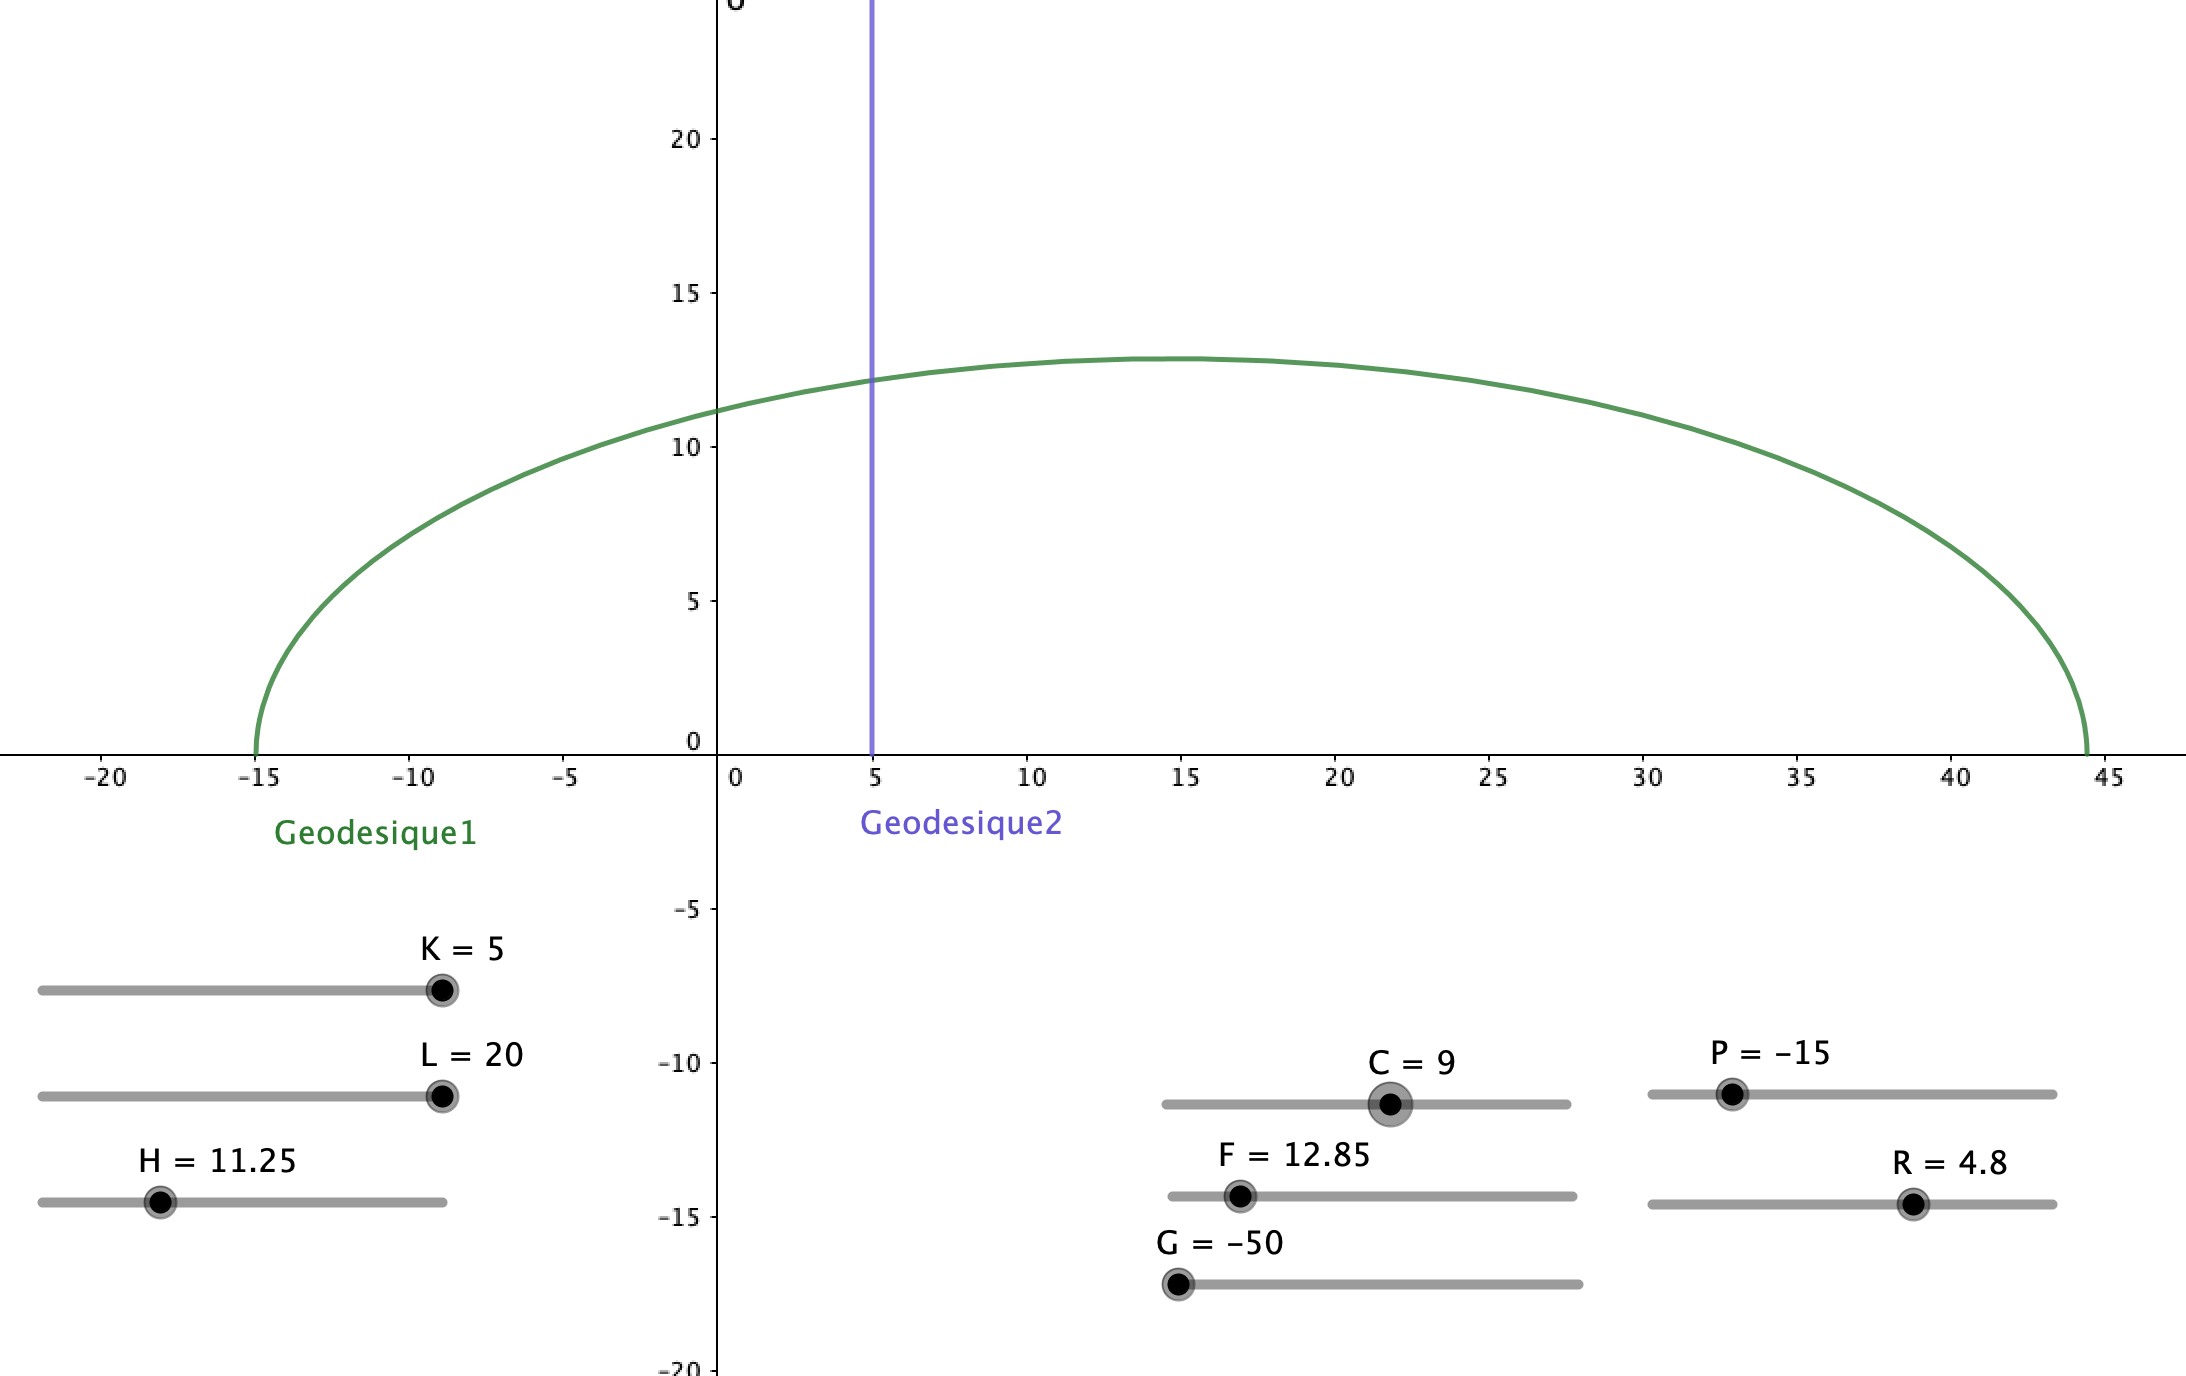
\includegraphics[scale=0.40]{image.png}
\end{center}    
avec $\mu$ sur l'axe des abcisses et $\sigma$ sur l'axe des ordonnées.\\     

Pour terminer la section, il est intéressant de noter, en passant, qu'avec la métrique standard sur $\mathbb{R}\times ]{0,+\infty[}$\footnote{Il est peut-être nécessaire de mentionner ici que sur $\mathbb{R}\times ]{0,+\infty[}$, appelé demi-plan de Poincaré, il existe une métrique standard appelée métrique hyperbolique et donnée, dans le cas qui nous concerne, par $\begin{bmatrix}
    \frac{1}{\sigma^2} & 0
    \\
    0 & \frac{1}{\sigma^2}
    \end{bmatrix}$.}, les géodésiques seraient des demi-droites verticales et des demi-cercles.\\



\section{Entropie de l'information et métrique de Fisher}
Supposons que l'on cherche à déterminer dans \eqref{my_manifold} la distribution la plus aléatoire, c'est-à-dire celle pour laquelle on dispose le moins d'information. Clairement, cette mesure  de l'incertitude devrait dépendre des paramètres. On appelle entropie une mesure du degré d'incertitude que présente une variable aléatoire et donc sa distribution de probabilité. On notera $H(p_{\xi}(x))=H(\xi)$ pour signifier l'entropie associée à la distribution $p_{\xi}$. Dans le cas où $x$ est une variable aléatoire continue, on la definie par (voir \cite[Section 3.2]{calin2014geometric}):
\begin{equation}\label{entropie}
    \begin{aligned}
    H\colon\mathbb{E} &\longrightarrow\mathbb{R} \\
    \xi &\longmapsto -E\left[\ln(p_{\xi})\right]=-\int_{-\infty}^{+\infty}p_{\xi}(x)\ln(p_{\xi}(x))dx 
\end{aligned}
\end{equation}

Pour une distribution normale de paramètres $\mu$ et $\sigma$, on peut aisément calculer ce que vaut l'entropie. On utilisant \eqref{entropie}, on a:
\begin{align*}
 H(\xi)&= -\int_{-\infty}^{+\infty}\left(\frac{1}{\sigma\sqrt{2\pi}}\exp\left(-\frac{(x-\mu)^2}{2\sigma^2}\right)\right)\left(-\ln\sigma\sqrt{2\pi}-\frac{(x-\mu)^2}{2\sigma^2}\right)dx\\
 &=\frac{\ln\sigma\sqrt{2\pi}}{\sigma\sqrt{2\pi}}\int_{-\infty}^{+\infty}\exp\left(-\frac{(x-\mu)^2}{2\sigma^2}\right)dx-\frac{1}{\sigma\sqrt{2\pi}}\int_{-\infty}^{+\infty}-\frac{(x-\mu)^2}{2\sigma^2}\exp\left(-\frac{(x-\mu)^2}{2\sigma^2}\right)dx\\
 &=\ln\sigma\sqrt{2\pi}-\frac{1}{2\sigma\sqrt{2\pi}}\left[\left.(x-\mu)\exp\left(-\frac{(x-\mu)^2}{2\sigma^2}\right)\right|_{-\infty}^{+\infty}-\int_{-\infty}^{+\infty}\exp\left(-\frac{(x-\mu)^2}{2\sigma^2}\right)dx\right]\\
 &=\ln\sigma\sqrt{2\pi}+\frac{1}{2}
\end{align*}
Observons qu'ici l'entropie ne dépend pas de $\mu$.
\newline

À présent, essayons de répondre à la question du début de la section. Il s'agit bien évidemment d'un problème de maximisation éventuellement sous contrainte selon que des observations auront apporté des éléments d'informations supplémentaires ou non. En clair, il s'agit de déterminer les points $p\in S$ où la fonction $H$ admet un maximum local. C'est d'abord un point critique en ce sens où la fonction $H$ devra satisfaire:
\begin{equation*}
    \frac{\partial H(\xi)}{\partial \xi_i}=0 \quad\text{pour}\quad i=1,2, \cdots, n
\end{equation*}
Mais c'est aussi un point où le hessien $hess(H)$ de $H$, c'est-à-dire la matrice des dérivées partielles secondes, $\frac{\partial^2 H(\xi)}{\partial \xi_j \partial\xi_ i}$, est définie négative au sens où $\langle hess(H), v \rangle<0$ \footnote{Ici, $\langle\;,\;\rangle$ est le produit scalaire} pour tout $v\in\mathbb{R}^n$. Les dérivées partielles secondes de $H$ se calculent par la formule suivante (voir \cite[Proposition 3.5.3]{calin2014geometric}):
\begin{equation}\label{entropie_metrique}
    \frac{\partial^2 H(\xi)}{\partial \xi_j \partial\xi_ i}=-g_{ij}(\xi)-h_{ij}(\xi)
\end{equation}
où $h_{ij}(\xi)=E\left[\frac{\partial\ln(p_{\xi})}{\partial\xi}\frac{\partial\ln(p_{\xi})}{\partial\xi_i}+\frac{\partial^2\ln(p_{\xi})}{\partial \xi_i \partial\xi_j}\ln(p_{\xi})\right]$.\\

Cette dernière équation \eqref{entropie_metrique} montre qu'il existe un lien entre la métrique de Fisher et l'entropie de l'information.\\

Terminons cette section par un résultat non trivial \cite[Théorème 6.5.1]{calin2014geometric}: parmi toutes les distributions sur $(-\infty, +\infty)$ de moyenne $\mu$ et d'écart-type $\sigma$ celle qui maximise l'entropie est la distribution normale. Si l'on se restreint au cas $\mu=0$ et $\sigma=1$ on voit alors que celle qui maximise l'entropie est:
\begin{equation*}
    p(x)=\frac{1}{\sqrt{2\pi}}\exp(-\frac{x^2}{2})
\end{equation*}
Si au lieu de travailler sur $(-\infty, +\infty)$ on travaille sur $(0, +\infty)$ on trouve une distribution exponentielle de la forme 
\begin{equation*}
    p(x)=\frac{1}{\mu}\exp(-\frac{x}{\mu})
\end{equation*}
et non la distribution normale!\\

\section{Divergence de \textit{Kullback-Leibler}}
En Géométrie de l'Information, il existe des mesures de distance qui ne possèdent toutes les pas la propriété de symétrie d'une métrique. On appelle de telles mesures des \textit{divergences} (voir \cite[Section 3.2]{amari2000nethods}). En particulier, une divergence sert à mesurer le "degré d'éloignement" (ou de rapprochement) de la distribution supposée (ou a priori) d'un ensemble d'observations par rapport à leur vraie loi de probabilité. Une divergence très utilisée est la divergence de \textit{Kullback-Leibler} aussi appelée entropie relative. Dans la suite, on se restreindra aux cas des variables aléatoires continues.

Soit $p_{\xi_p}(x)$ et $q_{\xi_q}(x)$ deux distributions continues de vecteurs de paramètres respectivement $\xi_p=(\mu_p, \sigma_p)$ et $\xi_q=(\mu_q, \sigma_q)$. On définit (voir \cite{calin2014geometric}) la divergence de \textit{Kullback-Leibler}, $D_{KL}$, entre les distributions $p_{\xi}(x)$ et $q_{\xi}(x)$ par:
\begin{equation*}
    D_{KL}(p||q)=E_{p_{\xi_p}}\left[\ln\frac{p_{\xi_p}(x)}{q_{\xi_q}(x)}\right]=\int_{-\infty}^{+\infty}p_{\xi_p}(x)\ln\frac{p_{\xi_p}(x)}{q_{\xi_q}(x)}dx
\end{equation*}\\
   
On peut illustrer le calcul de la divergence de \textit{Kullback-Leibler} pour deux distributions $p_{\xi_p}(x)=\frac{1}{\sigma_p\sqrt{2\pi}}\exp\left(-\frac{(x-\mu_p)^2}{2\sigma_p^2}\right)$ et $q_{\xi_q}(x)=\frac{1}{\sigma_q\sqrt{2\pi}}\exp\left(-\frac{(x-\mu_q)^2}{2\sigma_q^2}\right)$ sur la variété $S$ défine par \eqref  {my_manifold} où $q_{\xi_q}(x)$ comme la distribution a priori et $p_{\xi_p}(x)$ comme la vraie distribution. On a:

\begin{align*}
  D_{KL}(p||q)&=\int_{-\infty}^{+\infty}p_{\xi_p}(x)\ln\left(\frac{\frac{1}{\sigma_p\sqrt{2\pi}}\exp\left(-\frac{(x-\mu_p)^2}{2\sigma_p^2}\right)}{\frac{1}{\sigma_q\sqrt{2\pi}}\exp\left(-\frac{(x-\mu_q)^2}{2\sigma_q^2}\right)}\right)dx\\
  &=\int_{-\infty}^{+\infty}p_{\xi_p}(x)\left(-\ln\sigma_p\sqrt{2\pi}-\frac{(x-\mu_p)^2}{2\sigma_p^2}+\ln\sigma_q\sqrt{2\pi}+\frac{(x-\mu_q)^2}{2\sigma_q^2} \right)dx\\
  &=\ln\frac{\sigma_q}{\sigma_p}-\int_{-\infty}^{+\infty}\frac{(x-\mu_p)^2}{2\sigma_p^2}p_{\xi_p}(x)dx+\int_{+\infty}^{-\infty   }\frac{(x-\mu_q)^2}{2\sigma_q^2}p_{\xi_p}(x)dx\\
  &=\ln\frac{\sigma_q}{\sigma_p}-\frac{1}{2}+\int_{+\infty}^{-\infty   }\frac{(x-\mu_q)^2}{2\sigma_q^2}p_{\xi_p}(x)dx
\end{align*}
La troisième intégrale s'obtient en posant $\Delta\mu=\mu_p-\mu_q$ et en faisant les transformations nécessaires. D'où le résultat:
\begin{equation*}
   D_{KL}(p||q)=\ln\frac{\sigma_q}{\sigma_p}-\frac{1}{2}+\frac{\sigma_p^2+(\Delta\mu)^2}{2\sigma_q^2} 
\end{equation*}

Comme il fallait s'y attendre, lorsque les paramètres $\xi_q$ tendent vers $\xi_p$, $D_{KL}(p||q)$ tend vers zéro et la dérivée
\begin{equation*}
    \frac{\partial}{\partial\xi_i}D_{KL}(p||q)
\end{equation*}
y vaut également zéro.\\

Terminons par une relation qui montre le lien entre la divergence de \textit{Kullback-Leibler} et la métrique de Fisher. C'est celle-ci:
\begin{equation*}
    \left.\frac{\partial^2}{\partial\xi_i\partial\xi_j}\right|_{\xi_q=\xi_p}D_{KL}(p||q)=g_{ij}(\xi_p)\quad\text{pour}\quad i,j=1,2, \cdots, n
\end{equation*}
où $g_{ij}(\xi_p)$ est la $ij$-ème composante de la métrique $\textbf{g}_{ij}$ au point $p_{\xi_p}=(\mu_p, \sigma_p)$ et l'égalité $\xi_q=\xi_p$ signifie que la dérivée seconde est évaluée en $(\mu_p, \sigma_p)$. Dans le cas de notre variété $S$, on a voit bien que:
\begin{equation*}
    \frac{\partial^2D_{KL}(p||q)}{\partial\mu_p^2}=\frac{1}{\sigma_q^2}=g_{11},\;\frac{\partial^2D_{KL}(p||q)}{\partial\sigma_p\partial\mu_p}=\frac{\partial^2D_{KL}(p||q)}{\partial\mu_p\partial\sigma_p}=0\;\text{et}\;\frac{\partial^2D_{KL}(p||q)}{\partial\sigma_p^2}=\frac{2}{\sigma^2}=g_{22}
\end{equation*}\\\\


\renewcommand{\refname}{Références et bibliographie}
\bibliographystyle{plain}
\bibliography{References}	

\end{document} 
